\documentclass[11pt]{article}
\usepackage[margin=1in]{geometry}
\usepackage{booktabs}
\usepackage{array}
\usepackage{hyperref}
\usepackage{parskip}
\usepackage{enumitem}
\usepackage{xcolor}
\usepackage{tabularx}
\usepackage{amsmath}
\usepackage{natbib}
\usepackage{graphicx}
\usepackage{subcaption}
\usepackage{multirow}
\usepackage{textcomp}
\usepackage{amssymb}

\title{Model Selection Justification for the NAVIG Geolocalization Pipeline}
\author{Spencer Jenkins}
\date{\today}

\begin{document}
\maketitle

\tableofcontents
\bigskip

%----------------------------------------------------------------------
\section{Overview}
%----------------------------------------------------------------------

NAVIG~\citep{Yu2025NAVIG} is a multi-stage vision-language geolocalization pipeline. Given a
geo-tagged photograph, the system produces an estimated GPS coordinate---expressed as
(latitude, longitude, country, city)---by chaining six stages: (1)~macro-level scene reasoning,
(2)~visual grounding of salient objects via GroundingDINO~\citep{Liu2023GroundingDINO},
(3)~retrieval-augmented lookup against a geographic guidebook indexed with
CLIP~\citep{Radford2021CLIP} and FAISS~\citep{Johnson2021FAISS}, (4)~VLM-based commentary on
cropped patches, (5)~OCR-driven OpenStreetMap/Nominatim search, and (6)~final coordinate
synthesis. This document justifies the selection and configuration of every vision-language
model (VLM) used in these stages and reports an empirical evaluation that extends the
original paper in four directions the paper did not cover.

\paragraph{Why this evaluation extends the original paper.}
The original NAVIG paper evaluated three 7B-parameter SFT-trained models
(MiniCPM-V-2.6, LLaVA-1.6-Vicuna-7B, Qwen2-VL-7B) and reported their performance on
the GWS5k benchmark as the primary result, with im2gps3k results in the appendix.
The best result on im2gps3k was Navig-Qwen2-VL at GeoScore~3{,}482. The paper's
ablation study removed entire pipeline modules (Reasoner, Searcher) but did not
isolate the contribution of individual evidence types (RAG vs.\ patch commentary
vs.\ OSM). No experiment varied which model handled which stage: all three tested models
ran the full pipeline with their own SFT adapter, and no controlled Stage-6 swap
was performed. The paper identified four limitations---small training corpus,
street-view domain constraint, 7B model size ceiling, and pipeline component
conflicts---but provided no empirical diagnosis of which limitation most limits
performance.

This evaluation addresses those gaps directly:

\begin{enumerate}[noitemsep]
  \item \textbf{Evidence attribution:} A per-record analysis separates the
    contribution of RAG, patch commentary (COMMENT), and OSM evidence at the sample
    level---the first such decomposition for NAVIG. The finding that RAG
    \emph{systematically hurts} performance ($-356$ to $-756$ GeoScore points across
    all models) directly contradicts the original paper's implicit assumption that all
    Searcher components contribute positively.
  \item \textbf{Larger-model scaling:} LLaMA-3.2-11B is the first 11B-parameter
    model evaluated in the NAVIG pipeline. Its failure-excluded GeoScore of 3{,}357
    approaches the original paper's best result (Qwen2-VL SFT: 3{,}482), achieved
    without any NaviClues fine-tuning---a result with strong implications for whether
    SFT or raw model capacity is the primary performance driver.
  \item \textbf{Stage-level bottleneck isolation:} The Stage-6 swap experiment
    (Section~\ref{sec:swap}) is the first controlled test of whether Stage~6
    synthesis quality or Stage~1 reasoning quality is the performance bottleneck.
    This experiment is not present in any form in the original paper.
  \item \textbf{Geographic error analysis:} A regional breakdown (Section~\ref{sec:results})
    reveals a 47\% GeoScore gap between European images (3{,}205) and African images
    (1{,}686), quantifying the geographic bias that the original paper acknowledged as
    a qualitative limitation but did not measure.
\end{enumerate}

Our evaluation also replicates the original paper's LLaVA result closely
(2{,}626 vs.\ the paper's 2{,}592), confirming that the evaluation setup is consistent
with the original. Qwen2-VL---the original paper's strongest model---failed entirely in
our implementation due to a prompt-format incompatibility (Section~\ref{sec:failures})
that is diagnosed here and represents a concrete engineering target.

Three distinct experimental conditions are used across the model runs:

\begin{enumerate}[noitemsep]
  \item \textbf{Full pipeline with SFT} (primary models) --- a single model family drives
    both Stage~1 reasoning (via a LoRA-fine-tuned SFT variant~\citep{Hu2022LoRA}) and
    Stages~4--6 (via the same checkpoint loaded without the adapter). SFT is applied
    \emph{only} at Stage~1; Stages~4--6 always use the pretrained base weights.
  \item \textbf{Full pipeline, zero-shot} (comparison models) --- a model runs all six
    stages without any NAVIG-specific fine-tuning, providing zero-shot baselines that
    isolate the benefit of Stage~1 SFT.
  \item \textbf{Stage-6 swap only} --- the pre-computed Stage-1--5 outputs from the LLaVA
    full-pipeline run are held fixed, and a different model is substituted exclusively at
    Stage~6. This tests whether coordinate synthesis quality is the primary bottleneck,
    independent of upstream evidence generation.
\end{enumerate}

Table~\ref{tab:summary} summarises all seven model configurations and their experimental roles.

\begin{table}[ht]
\centering
\caption{Model inventory, experimental roles, and evaluation status.
         ``SFT'' indicates that a LoRA adapter fine-tuned on NaviClues is applied
         at Stage~1; all other stages always use pretrained base weights.
         \dag~LLaMA-3.2-11B is the only model evaluated in both the full-pipeline
         and Stage-6-swap conditions.
         \ddag~InternVL2-8B was implemented and is described in
         Section~\ref{sec:cmp}, but has not yet been evaluated.}
\label{tab:summary}
\begin{tabularx}{\textwidth}{llllXl}
\toprule
\textbf{Class name(s)} & \textbf{Checkpoint} & \textbf{Params} & \textbf{Condition} & \textbf{Role(s)} & \textbf{SFT?} \\
\midrule
\texttt{LLaVA} / \texttt{LLaVA\_sft} & LLaVA-1.6-Vicuna-7B           & 7B  & Full pipeline (SFT)    & Stage~1 (SFT), Stages~4--6 (base) & Stage~1 only \\
\texttt{Qwen} / \texttt{Qwen\_sft}   & Qwen2-VL-7B-Instruct          & 7B  & Full pipeline (SFT)    & Stage~1 (SFT), Stages~4--6 (base) & Stage~1 only \\
\texttt{CPM} / \texttt{CPM\_sft}     & MiniCPM-V-2.6                 & 8B  & Full pipeline (SFT)    & Stage~1 (SFT), Stages~4--6 (base) & Stage~1 only \\
\texttt{Llama32Vision}\dag            & Llama-3.2-11B-Vision-Instruct & 11B & Full pipeline + swap   & All stages (zero-shot); also Stage~6 swap & No \\
\texttt{DeepSeekVL}                  & DeepSeek-VL-7B-Chat           & 7B  & Full pipeline          & All stages (zero-shot)            & No \\
\texttt{FalconVLM}                   & Falcon-11B-VLM                & 11B & Full pipeline          & All stages (zero-shot)            & No \\
\texttt{InternVL2}\ddag              & InternVL2-8B                  & 8B  & Planned (not run)      & ---                               & No \\
\bottomrule
\end{tabularx}
\end{table}

%----------------------------------------------------------------------
\section{Evaluation Dataset: im2gps3k}
\label{sec:im2gps3k}
%----------------------------------------------------------------------

All experiments in this document are evaluated on the \textbf{im2gps3k} benchmark,
introduced by \citet{Vo2017IM2GPS3K} as a harder, larger complement to the original
237-image IM2GPS test set of \citet{Hays2008IM2GPS}. The dataset consists of
2{,}997 GPS-tagged photographs sourced from Flickr---the same community photograph
platform used to construct the underlying IM2GPS retrieval database---but without
the manual curation applied to the original test set. This deliberate absence of
filtering means im2gps3k contains the full range of image types submitted by real
photographers: recognisable landmarks, urban street scenes, rural and natural
landscapes, wildlife photographs, and close-up subject photography. The challenge
of geo-localization on this benchmark reflects the challenge of geo-localization in
the real world.

\paragraph{Geographic distribution.}
As shown in Figure~\ref{fig:dataset_geo}, the dataset is strongly biased toward
Western-hemisphere photographers: Europe accounts for 35.6\% (1{,}067 images) and
North America for 31.2\% (936 images), together representing two-thirds of the
benchmark. Asia contributes 15.2\% (455 images), while Africa (5.3\%), South
America (3.8\%), and Oceania (1.4\%) are heavily under-represented relative to
their landmass or population. A further 7.5\% of images do not fall within the
defined continental bins (polar regions, island chains, or ambiguous coordinates).
This distribution directly mirrors the geographic bias of Flickr's userbase in the
benchmark's collection window, and it has two important consequences for evaluation:
(1)~models will see more training-distribution-similar content in European and North
American test images, inflating aggregate metrics; and (2)~reported performance on
under-represented regions is computed over small sample sizes and therefore has high
variance.

\begin{figure}[ht]
  \centering
  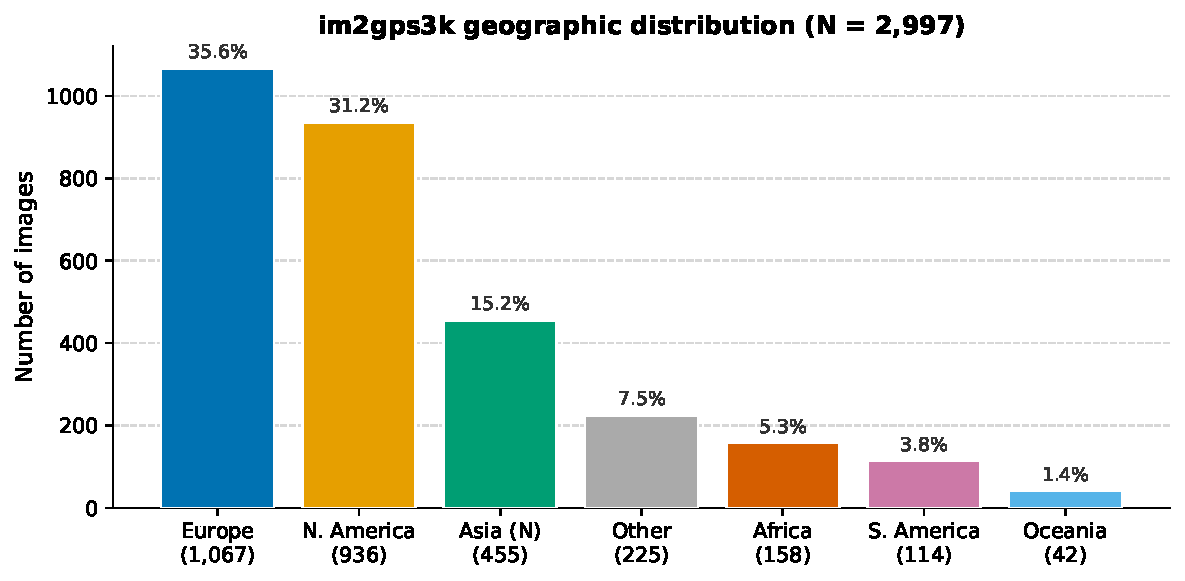
\includegraphics[width=0.82\textwidth]{figures/fig_dataset_geo.pdf}
  \caption{Geographic distribution of the 2{,}997-image im2gps3k benchmark by
           broad continental region. Europe and North America together account for
           two-thirds of the dataset, reflecting the geographic bias of Flickr
           photographers in the collection window.}
  \label{fig:dataset_geo}
\end{figure}

\paragraph{Image content and difficulty.}
The benchmark spans at least four qualitatively distinct image categories, each
presenting a different failure mode for the NAVIG pipeline:

\begin{enumerate}[noitemsep]
  \item \textbf{Landmark photographs.} Images of globally recognisable structures
    (the Eiffel Tower, Trafalgar Square, the Taj Mahal) can be localised to within
    metres by VLMs that have learned to associate these structures with specific
    GPS coordinates from pretraining data. These images are trivially easy and
    inflate aggregate accuracy at fine-grained thresholds.

  \item \textbf{Text-bearing urban scenes.} Street scenes containing legible local
    text---shop signs, road signs, street name plates---can be localised by the
    OCR+Nominatim chain in Stage~5, provided the text is in a language or script
    with distinctive geographic specificity (Arabic, Cyrillic, Thai, etc.).

  \item \textbf{Generic urban infrastructure.} Parking lots, plain building
    facades, and undistinctive roadways carry subtle visual cues---bollard
    colours, road marking styles, kerb design, licence plate proportions---that
    human experts (e.g.\ GeoGuessr players) can read but current VLMs frequently
    misinterpret. These images produce the hemisphere-flipping errors visible in
    Figure~\ref{fig:dataset_examples} (left, bottom row): the model correctly
    identifies a temperate-climate English-speaking country but places it on the
    wrong side of the Earth.

  \item \textbf{Natural landscapes and subject photography.} Images showing
    wildlife, close-up flora, or featureless natural terrain provide little or no
    geographic signal for a VLM operating at the text-prompt level. The pipeline
    can only hallucinate a species-based geographic prior (e.g.\ associating a
    crocodile photograph with Cuba rather than Thailand) or default to a polar
    confusion when confronted with a barren volcanic landscape. No amount of
    upstream SFT or downstream RAG retrieval can recover meaningful localisation
    from an image that contains no geographic information.
\end{enumerate}

Figure~\ref{fig:dataset_examples} illustrates the contrast between categories~1
and~4 concretely, comparing three near-perfect predictions against three
maximum-error failures from the LLaVA-1.6 full pipeline. The
failures are not random: they are predictable from the image content alone. This
is an important caveat when interpreting aggregate GeoScore numbers---a model that
achieves GeoScore~2626 is not ``26\% of optimal'' uniformly; it is very good
at landmark images and completely uninformative on a systematic subset of the
benchmark.

\begin{figure}[p]
  \centering
  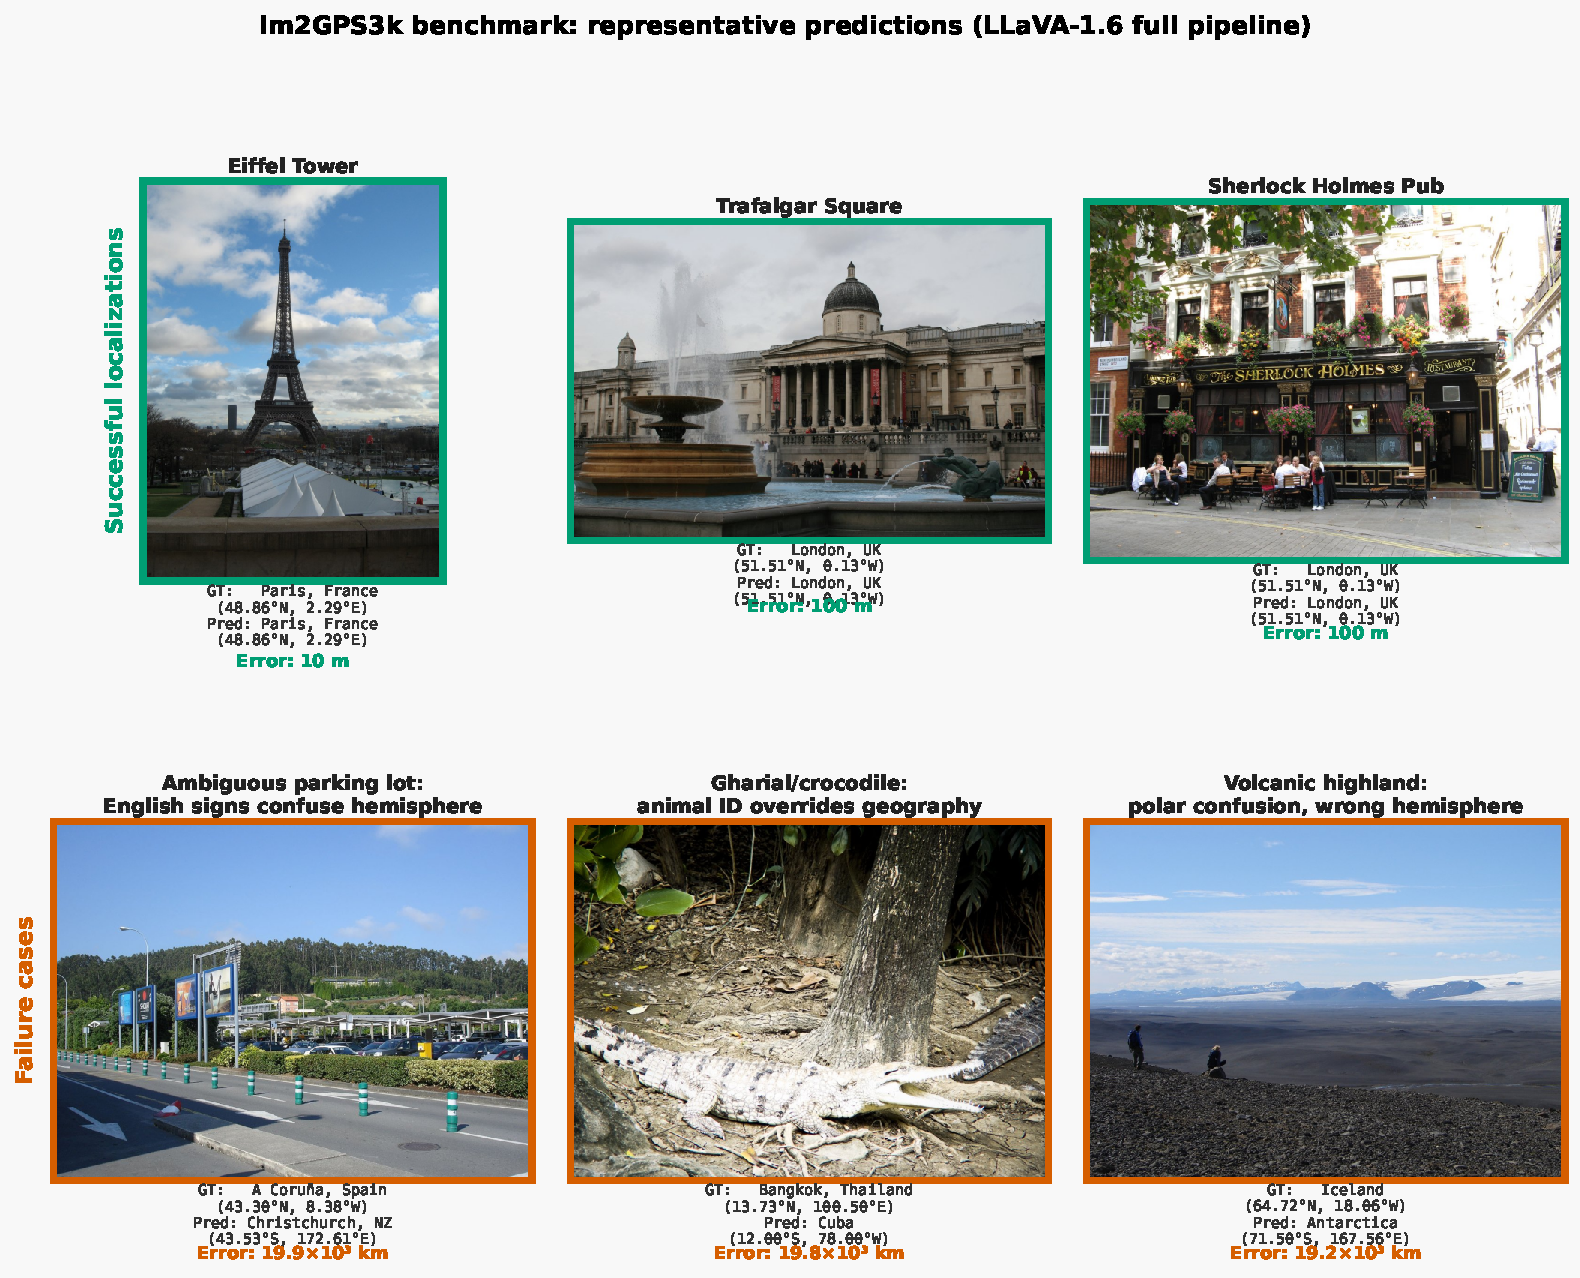
\includegraphics[width=\textwidth]{figures/fig_dataset_examples.pdf}
  \caption{Representative im2gps3k predictions from the LLaVA-1.6 full pipeline.
    \textbf{Top row (successes):} Landmark-rich images are localised to within
    metres. Left: Eiffel Tower (Paris), 0.01\,km error.
    Centre: National Gallery, Trafalgar Square (London), 0.10\,km error.
    Right: The Sherlock Holmes pub, Northumberland Street (London), 0.10\,km
    error---the pub name and street sign are both legible, making it trivially
    identifiable.
    \textbf{Bottom row (failures):} Images providing little or no geographic
    signal produce antipodal errors exceeding 19{,}000\,km.
    Left: A commercial parking area in A~Coru\~{n}a, Spain; English-language
    signage and temperate greenery caused the model to predict Christchurch,
    New Zealand (19{,}931\,km error).
    Centre: A gharial photographed in Bangkok, Thailand; the model associated the
    species with Cuba (19{,}763\,km error).
    Right: The Icelandic highland near M\'{y}rdalsjokull; the barren volcanic terrain
    and distant glacier were interpreted as Antarctica (19{,}226\,km error).
    The failure cases are categorically different from the successes---they contain
    almost no unambiguous geographic signal---and represent a systematic, not
    random, source of error.}
  \label{fig:dataset_examples}
\end{figure}

\paragraph{Suitability for NAVIG evaluation.}
im2gps3k was selected as the primary evaluation benchmark for three reasons.
First, the original NAVIG paper~\citep{Yu2025NAVIG} reported results on im2gps3k,
making it the natural choice for assessing comparability with prior work.
Second, at 2{,}997 images it is large enough to support statistically meaningful
breakdown by geographic region and evidence type, as reported in
Section~\ref{sec:results}. Third, the benchmark is old enough (images collected
before $\sim$2017) that it is unlikely to have been included in the pretraining
corpora of the VLMs evaluated here, reducing the risk of inadvertent memorisation.

A known limitation is that im2gps3k over-represents landmark and tourist imagery
relative to the realistic distribution of geo-localization queries in deployment.
This inflates reported accuracy at fine-grained distance thresholds (1\,km and
25\,km) relative to what a deployed system would achieve on arbitrary queries.
Future work should include evaluation on GWS15K, which has a more uniform
geographic distribution, and on street-level datasets closer in character to
GeoGuessr gameplay---the domain on which the Stage~1 models were fine-tuned.

%----------------------------------------------------------------------
\section{Training Dataset: NaviClues}
\label{sec:navclues}
%----------------------------------------------------------------------

The Stage~1 reasoning models are fine-tuned on \textbf{NaviClues}, a proprietary
dataset of geolocalization gameplay transcripts collected from expert GeoGuessr
players and paired with the photographs they were shown. Each record stores an image
path, a YouTube gameplay URL, the GeoGuessr challenge URL, the ground-truth GPS
coordinate, a timestamped player commentary transcript, the GeoScore awarded
(0--5000 points on the standard exponential scale), and the Haversine error in
kilometres. Images are hosted publicly on Hugging~Face at
\texttt{huggingCode11/NAVICLUES}; LoRA adapters are at \texttt{huggingCode11/NAVIG}.

The raw corpus contains 2{,}637 samples, filtered to 1{,}638 samples after quality
and diversity screening (\texttt{filtered\_data.jsonl}), and further refined to
390 high-quality samples (\texttt{quality\_data.jsonl}) used for the final SFT runs.
This aggressive 85\% reduction reflects the difficulty of extracting clean
training signal from unstructured gameplay video: many transcripts are incomplete,
redundant, or contain irrelevant commentary. The 390 retained samples are those
where the player's verbal reasoning is geographically specific, internally
consistent, and achieves a GeoScore above a quality threshold.

The GeoScore metric used for both training-data selection and evaluation follows the
standard exponential decay formula from the original NAVIG paper:
\begin{equation}
  \label{eq:geoscore}
  \mathrm{GeoScore}(d) = 5000 \cdot \exp\!\Bigl(-\frac{d}{1492.7}\Bigr),
\end{equation}
where $d$ is the Haversine distance in kilometres between the predicted and
ground-truth coordinates. A score of 5000 indicates a perfect prediction;
a score of~0 corresponds to a prediction on the opposite side of the globe
($d \gtrsim 10{,}000$\,km).

\paragraph{NaviClues vs.\ im2gps3k: domain mismatch.}
NaviClues images derive from GeoGuessr gameplay, which uses Google Street View
panoramas---near-ground-level, 360-degree imagery collected by dedicated camera
rigs under standardised exposure. im2gps3k images are amateur Flickr photographs
with arbitrary composition, exposure, and subject matter. The Stage~1 model is
therefore fine-tuned on a somewhat different visual domain than the one it is
evaluated on. This domain gap is one reason why the SFT benefit---while real---is
more modest than might be expected from the quality of the training transcripts.
Closing this gap, by augmenting NaviClues with Flickr-style imagery or by
fine-tuning directly on a sample of im2gps3k images, is a concrete avenue for
future improvement.

%----------------------------------------------------------------------
\section{Fine-Tuning and Inference Infrastructure}
\label{sec:infra}
%----------------------------------------------------------------------

All SFT runs use the \textbf{ms-Swift} framework~\citep{msSwift2024} (version 2.5.0.post1)
with LoRA adapters~\citep{Hu2022LoRA} of rank~16. Training converges at step~534 for each
model family, producing the shared \texttt{checkpoint-534} naming convention visible in
the \texttt{vlms/} directory. At inference time, the \texttt{\_sft} variant loads the
pretrained weights and then applies the saved LoRA checkpoint via
\texttt{Swift.from\_pretrained(\ldots, inference\_mode=True)}.

The pipeline runs on single NVIDIA RTX A6000 GPUs (48\,GB VRAM, compute capability SM~8.6)
under CUDA~12.1 and PyTorch~2.4.0. All models are loaded in \texttt{float16} (except
InternVL2-8B, which uses \texttt{bfloat16} for numerical stability as recommended by the
model authors). To avoid holding two copies of a 7\,B model in VRAM simultaneously, the
reasoning model (Stage~1) is loaded, used, and freed before the base model (Stages~4--6)
is instantiated. The SFT model always uses the ms-Swift inference path regardless of
runtime flags, because vLLM's multimodal LoRA support for LLaVA-NeXT is not yet stable.

Optional vLLM~\citep{Kwon2023vLLM} acceleration (version~0.5.5) is available for
Stages~4--6 via the \texttt{--use\_vllm} flag. vLLM applies \emph{only} to the base model
in these later stages; Stage~1 always falls back to ms-Swift.

For visual grounding (Stage~2), NAVIG uses GroundingDINO~\citep{Liu2023GroundingDINO} with
a Swin-T backbone (\texttt{groundingdino\_swint\_ogc.pth}), configured by default with
box threshold 0.65 and text threshold 0.55, detecting three object categories: road signs,
house facades, and building signs. Stage~3 retrieval is built on CLIP
ViT-B/32~\citep{Radford2021CLIP} embeddings over a curated geographic guidebook, stored in
a FAISS~\citep{Johnson2021FAISS} L2 index; the distance threshold for including a retrieved
clue in the Stage~6 prompt is set to 30 (L2 units in the embedding space).

%----------------------------------------------------------------------
\section{Primary Pipeline Models (with Supervised Fine-Tuning)}
\label{sec:primary}
%----------------------------------------------------------------------

The three models below are the core subjects of NAVIG's supervised fine-tuning study.
Each was fine-tuned on the 390-sample NaviClues quality subset using LoRA adapters managed
by ms-Swift, as described in Section~\ref{sec:infra}.

%----------------------------------
\subsection{LLaVA-1.6-Vicuna-7B (\texttt{LLaVA} / \texttt{LLaVA\_sft})}
%----------------------------------

\textbf{Architecture.} LLaVA-NeXT (version~1.6)~\citep{Liu2024LLaVANeXT}, which builds
on LLaVA-1.5~\citep{Liu2024LLaVA15}, couples a CLIP ViT-L/14@336px vision
encoder~\citep{Radford2021CLIP} with Vicuna-7B~\citep{Chiang2023Vicuna} as the language
backbone. Images are tiled into up to six high-resolution patches (a 2$\times$2 grid plus
one global thumbnail) before being projected into the language embedding space, giving the
model substantially finer spatial resolution than the LLaVA-1.5 family. The ms-Swift model
type is \texttt{llava1\_6-vicuna-7b-instruct}; the LLaVA-NeXT processor requires the
\texttt{patch\_size} and \texttt{vision\_feature\_select\_strategy} attributes to be set
explicitly (patched in \texttt{llm.py::\_fix\_llava\_next\_processor} to avoid an upstream
deprecation warning in transformers~4.45.2).

\textbf{Why chosen.} LLaVA-1.6-Vicuna-7B served as the original baseline model in the
first published iteration of NAVIG~\citep{Yu2025NAVIG}. Its inclusion is therefore both a
continuity decision---preserving direct comparability with prior published numbers---and an
architectural one: the tile-based high-resolution encoding is well-suited to street-level
images containing small but legible signs and text. At 7\,B parameters the model fits
comfortably within a single 48\,GB A6000 GPU in \texttt{float16} ($\approx$14\,GB VRAM).

\textbf{Fine-tuning.} A LoRA adapter (rank~16) was trained on the NaviClues quality subset
and is stored at \texttt{vlms/NAVIG/llava1\_6-vicuna-7b-instruct/checkpoint-534}. The SFT
variant (\texttt{LLaVA\_sft}) is used \emph{only} in Stage~1 to generate the macro
geographic reasoning chain. The base model (\texttt{LLaVA}) handles Stages~4--6 without the
adapter.

\textbf{vLLM path.} An optional \texttt{LLaVA\_vllm} / \texttt{LLaVA\_sft\_vllm} path
accelerates throughput via vLLM with LoRA pass-through. Because vLLM's multimodal LoRA
support for LLaVA-NeXT is not fully stable, vLLM is applied \emph{only} to the base model
when \texttt{--use\_vllm} is set; Stage~1 always uses the ms-Swift path.

%----------------------------------
\subsection{Qwen2-VL-7B-Instruct (\texttt{Qwen} / \texttt{Qwen\_sft})}
%----------------------------------

\textbf{Architecture.} Qwen2-VL-7B~\citep{Wang2024Qwen2VL} is Alibaba's second-generation
visual language model. It introduces a \emph{Naive Dynamic Resolution} mechanism that allows
the vision encoder to process images at their native aspect ratio and resolution rather than
forcing a fixed square crop, and a \emph{Multimodal Rotary Position Embedding} (M-RoPE)
that jointly encodes spatial and temporal positions across the image and text sequence. The
language backbone is Qwen2-7B. The ms-Swift model type is \texttt{qwen2-vl-7b-instruct};
weights from the subsequent Qwen2.5-VL release (which shares the same architecture and
tokeniser) are forward-compatible with this model type in ms-Swift.

\textbf{Why chosen.} Qwen2-VL-7B achieves strong performance on OCR and document
understanding benchmarks (e.g., TextVQA, OCRBench, DocVQA) relative to comparably sized
models~\citep{Wang2024Qwen2VL}. This is directly relevant to Stages~4--5 of NAVIG, which
rely on reading small cropped text patches---signs, storefronts, road markings---to generate
Nominatim search queries. Qwen2-VL's native-resolution encoding is particularly advantageous
when patches are non-square or of variable aspect ratio, as is typical of GroundingDINO
detections.

\textbf{Fine-tuning.} A LoRA adapter was trained under the same procedure as LLaVA and is
stored at \texttt{vlms/qwen/checkpoint-534}. The \texttt{Qwen\_sft} variant drives Stage~1;
\texttt{Qwen} (base) drives Stages~4--6.

%----------------------------------
\subsection{MiniCPM-V-2.6 (\texttt{CPM} / \texttt{CPM\_sft})}
%----------------------------------

\textbf{Architecture.} MiniCPM-V-2.6~\citep{Yao2024MiniCPMV} is a compact multimodal model
from ModelBest/OpenBMB. It is built around the SigLIP-400M vision
encoder~\citep{Zhai2023SigLIP} and the Qwen2-7B language model, totalling approximately
8\,B parameters. It employs an adaptive visual encoding scheme and an efficient \emph{token
compression} mechanism that reduces the number of visual tokens passed to the language model,
enabling longer effective context at lower memory cost. MiniCPM-V-2.6 additionally supports
native multi-image input in a single forward pass. The ms-Swift model type is
\texttt{minicpm-v-v2\_6-chat}.

\textbf{Why chosen.} MiniCPM-V-2.6 offers a different architecture trade-off than LLaVA and
Qwen: aggressive visual token compression reduces VRAM pressure during Stage~4's multi-patch
commenting loop, and the native multi-image interface is directly relevant to stages that
process batches of crops. Including MiniCPM tests whether the visual understanding bottleneck
in NAVIG lies in image encoding quality (favouring Qwen or LLaVA) or in token-efficient
summarisation (favouring MiniCPM). The SigLIP-400M encoder is trained with a sigmoid loss
rather than a contrastive softmax, which empirically improves performance at smaller batch
sizes~\citep{Zhai2023SigLIP}.

\textbf{Fine-tuning.} A LoRA adapter was trained identically to the other primary models
and is stored at \texttt{vlms/cpm/checkpoint-534}. The \texttt{CPM\_sft} variant drives
Stage~1; \texttt{CPM} drives Stages~4--6.

%----------------------------------------------------------------------
\section{Full-Pipeline Comparison Models (Zero-Shot, No SFT)}
\label{sec:cmp}
%----------------------------------------------------------------------

The three models in this section were each run through the \emph{complete} six-stage
NAVIG pipeline---all stages 1--6---without any NAVIG-specific fine-tuning. Each model
therefore generated its own Stage~1 geographic reasoning chain, performed its own
Stage~4 patch commentary, and synthesised its own Stage~6 coordinate prediction,
all zero-shot from pretrained base weights. This design isolates the benefit of the
Stage~1 LoRA adapter: comparing these zero-shot full-pipeline runs against the
SFT-trained primary models (Section~\ref{sec:primary}) directly measures how much
NaviClues fine-tuning improves end-to-end accuracy when the same model family is
held constant.

Each model was selected to vary a distinct architectural axis relative to the primary
models: parameter scale (7B vs.\ 11B), visual encoding strategy (tile-based
vs.\ dual-encoder), language backbone, and pretraining data distribution. A fourth
comparison model, InternVL2-8B (implemented in \texttt{llm.py} and described in
Section~\ref{sec:internvl2}), was planned under the same design but has not yet been
evaluated due to scheduling constraints.

\paragraph{Relationship to the Stage-6 swap experiment.}
Separately from the full-pipeline comparison runs, a \emph{Stage-6 swap} experiment
was conducted using \texttt{guess\_only.py} (Section~\ref{sec:swap}). In that
experiment, the pre-computed Stage~1--5 outputs from the LLaVA full-pipeline run
are held fixed, and LLaMA-3.2-11B-Vision-Instruct is substituted at Stage~6 only.
LLaMA-3.2 is therefore the only model evaluated in both conditions---as a full-pipeline
model generating its own upstream evidence, and as a Stage~6 guesser operating on
LLaVA's upstream evidence. The comparison between these two conditions
(Sections~\ref{sec:results} and~\ref{sec:discussion}) directly tests whether the
upstream reasoning chain or Stage~6 synthesis quality is the performance bottleneck.

%----------------------------------
\subsection{Llama-3.2-11B-Vision-Instruct (\texttt{Llama32Vision})}
%----------------------------------

\textbf{Architecture.} Meta's Llama-3.2-11B-Vision-Instruct~\citep{Meta2024Llama3} grafts a
cross-attention vision adapter onto a Llama~3.1 text backbone, scaling the combined model to
11\,B parameters. The cross-attention fusion mechanism integrates visual features at multiple
decoder layers rather than projecting them solely at the input, and the model was
instruction-tuned specifically for visual question answering and visual reasoning tasks. The
ms-Swift model type is \texttt{llama3\_2-11b-vision-instruct}.

\textbf{Why chosen.} At 11\,B parameters, LLaMA-3.2-11B is the largest model in the
comparison set. It is hypothesised to have the strongest geographic commonsense reasoning
capability, owing to the larger Llama~3.1 pretraining corpus~\citep{Meta2024Llama3}, and
is accordingly recommended as the default zero-shot model in the experimental workflow
(see \texttt{guess\_only.py}). At \texttt{float16} it requires approximately 22\,GB of
VRAM, fitting comfortably on a single 48\,GB A6000 card.

\textbf{Fine-tuning.} Not fine-tuned. Runs the full pipeline zero-shot for all stages.
Also used in the Stage-6 swap experiment (\texttt{guess\_only.py}), where it receives
LLaVA's pre-generated Stage~1--5 outputs and synthesises only the final coordinate.

%----------------------------------
\subsection{DeepSeek-VL-7B-Chat (\texttt{DeepSeekVL})}
%----------------------------------

\textbf{Architecture.} DeepSeek-VL-7B-Chat~\citep{Lu2024DeepSeekVL} from DeepSeek AI uses a
hybrid visual encoder that combines a \emph{low-resolution} SigLIP-L branch
(384$\times$384)~\citep{Zhai2023SigLIP} for global context with a \emph{high-resolution}
SAM-ViT-B branch (1024$\times$1024)~\citep{Kirillov2023SAM} for fine-grained spatial detail,
concatenating their output features before projection into the language model. The language
backbone is DeepSeek-LLM-7B-base. This dual-encoder design was motivated by the empirical
finding that high-resolution and low-resolution encoders capture complementary spatial
features~\citep{Lu2024DeepSeekVL}. The ms-Swift model type is \texttt{deepseek-vl-7b-chat}.

\textbf{Why chosen.} DeepSeek-VL-7B serves as a 7\,B full-pipeline baseline with a
qualitatively different visual architecture from the SFT models. Its dual-encoder design
(global SigLIP-L + high-resolution SAM-ViT-B) provides a wider effective receptive field
than either the tiled CLIP approach (LLaVA) or the native-resolution Qwen ViT. At the same
parameter count as LLaVA and Qwen, any performance difference is attributable to the
architecture and training distribution rather than capacity.

\textbf{Fine-tuning.} Not fine-tuned. Runs the full pipeline zero-shot for all stages.

%----------------------------------
\subsection{Falcon-11B-VLM (\texttt{FalconVLM})}
%----------------------------------

\textbf{Architecture.} Falcon-11B-VLM from the Technology Innovation Institute is built on
the LLaVA-NeXT framework~\citep{Liu2024LLaVANeXT} with Falcon-11B~\citep{Almazrouei2023Falcon}
as the language backbone replacing Vicuna. It uses \texttt{LlavaNextProcessor} and
\texttt{LlavaNextForConditionalGeneration} from HuggingFace Transformers, retaining the same
CLIP ViT-L/14 vision encoder and tile-based high-resolution encoding as LLaVA-1.6-Vicuna-7B.
Falcon-11B was pretrained on the RefinedWeb dataset~\citep{Almazrouei2023Falcon}, a large,
heavily deduplicated English web corpus, giving it a substantially different pretraining
distribution from Vicuna, Qwen2, or Llama.

\textbf{Why chosen.} Falcon-11B-VLM is the controlled counterpart to LLaVA-1.6-Vicuna-7B
in the full-pipeline comparison. The two models share nearly identical visual architectures
(CLIP ViT-L/14, LLaVA-NeXT tiling) but differ in language backbone and parameter count.
Running both through the full pipeline with no SFT isolates whether the performance gap
between them---if any---is attributable to the language backbone (Falcon vs.\ Vicuna) or to
the Stage~1 SFT adapter that the primary LLaVA run carries.

\textbf{Integration note.} Unlike the other comparison models, ms-Swift does not natively
support Falcon-11B-VLM, so the \texttt{FalconVLM} class uses the raw
\texttt{LlavaNextProcessor} / \texttt{LlavaNextForConditionalGeneration} API directly. Two
compatibility patches are applied at runtime: (1)~the embedding matrix is resized to cover
the \texttt{<image>} special token at index~65024 (the saved matrix had only 65024 rows,
causing out-of-bounds CUDA errors during lookup); and (2)~a forward-compatibility shim
removes the \texttt{num\_logits\_to\_keep} keyword argument that the installed
\texttt{FalconForCausalLM} predates.

\textbf{Fine-tuning.} Not fine-tuned. Runs the full pipeline zero-shot for all stages.

%----------------------------------
\subsection{InternVL2-8B (\texttt{InternVL2}) --- Planned}
\label{sec:internvl2}
%----------------------------------

\textbf{Architecture.} InternVL2-8B~\citep{Chen2024InternVL} from OpenGVLab pairs
InternViT-300M-448px (a 300\,M-parameter vision transformer fine-tuned for 448\,px
dynamic-tiling input via a progressive alignment curriculum) with InternLM2-7B as
the language backbone, for a combined 8\,B parameters. The progressive alignment strategy
first trains the vision encoder in isolation, then jointly trains the cross-modal
projection, yielding particularly strong performance on OCR-heavy and document
understanding benchmarks. In NAVIG it is loaded in \texttt{bfloat16}, matching the
numerical format recommended by the model authors. The ms-Swift model type is
\texttt{internvl2-8b}.

\textbf{Why chosen.} InternVL2-8B is the only comparison model with a vision encoder
trained specifically under a supervised \emph{visual} alignment curriculum rather than
contrastive (CLIP-style) or sigmoid (SigLIP-style) pre-training. Its superior OCR
grounding is hypothesised to benefit Stages~4--5 (patch commentary, Nominatim query
generation) more than any other comparison model, providing a cleaner test of whether
text-reading quality---rather than geographic reasoning---is the primary bottleneck.
InternVL2 is fully implemented in \texttt{llm.py} and ready to evaluate; scheduling
constraints have delayed its full-pipeline run.

\textbf{Fine-tuning.} Not fine-tuned. Will be run zero-shot for all stages.
\textbf{Evaluation status: not yet run.}

%----------------------------------------------------------------------
\section{Stage-6 Swap Experiment}
\label{sec:swap}
%----------------------------------------------------------------------

Beyond the full-pipeline runs described above, a dedicated Stage-6 swap experiment
was conducted via \texttt{guess\_only.py}. In this design, the pipeline is run in
two passes: first, the LLaVA full-pipeline run (Section~\ref{sec:primary}) generates
Stage~1--5 outputs for all 2{,}997 images and saves them to
\texttt{results\_s5.jsonl}; second, \texttt{guess\_only.py} loads those cached
outputs and passes the full structured prompt---Stage~1 reasoning chain, RAG clues,
Stage~4 patch commentary, and Stage~5 Nominatim results---to a different model for
Stage~6 coordinate synthesis only.

This design is distinct from the full-pipeline comparison runs in a critical way:
the upstream evidence chain is \emph{held constant} across the swap. Any change in
final GeoScore therefore reflects Stage~6 synthesis quality alone, not differences
in Stage~1 reasoning or patch commentary. LLaMA-3.2-11B-Vision-Instruct was chosen
as the swap model because it is the strongest available zero-shot guesser and is
the model recommended for this role in the codebase.

The Stage-6 swap experiment tests two explicit hypotheses:
\begin{itemize}[noitemsep]
  \item \textbf{H1}: The bottleneck is Stage~1 reasoning quality (the SFT adapter).
    Under H1, the Stage-6 swap should produce similar or worse results than the
    LLaVA baseline, since Stage~1 is unchanged and Stage~6 is not the limiting factor.
  \item \textbf{H2}: The bottleneck is Stage~6 synthesis quality (coordinate
    regression from the prompt). Under H2, substituting a stronger Stage~6 model
    should substantially improve GeoScore.
\end{itemize}
Results and interpretation are provided in Section~\ref{sec:discussion}.

%----------------------------------------------------------------------
\section{Architectural Comparison}
%----------------------------------------------------------------------

Table~\ref{tab:diff} provides a side-by-side architectural summary of all seven
model configurations. Each row highlights the feature axis that motivated that
model's inclusion: vision encoder design, language backbone, inference backend
constraint, or a specific capability hypothesis (OCR quality, dual-resolution
encoding, language-model capacity). Read in conjunction with the per-model
subsections above, this table makes explicit which experimental variables are
held constant and which are varied across the swap experiment.

\begin{table}[ht]
\centering
\caption{Architectural summary and experimental condition for all seven model
         configurations. Primary models (rows 1--3) use an SFT adapter at Stage~1;
         comparison models (rows 4--7) run the full pipeline zero-shot.
         LLaMA-3.2-11B additionally appears in the Stage-6 swap experiment.
         InternVL2-8B is implemented but not yet evaluated (\S\ref{sec:internvl2}).}
\label{tab:diff}
\begin{tabularx}{\textwidth}{lXXXl}
\toprule
\textbf{Model} & \textbf{Vision encoder} & \textbf{Language backbone} & \textbf{Distinguishing feature} & \textbf{Inference backend} \\
\midrule
\multicolumn{5}{l}{\emph{Primary models — full pipeline with Stage-1 SFT}} \\
\midrule
LLaVA-1.6-Vicuna-7B & CLIP ViT-L/14@336px (tiled) & Vicuna-7B    & Original NAVIG baseline; tile-based HR encoding  & ms-Swift / vLLM \\
Qwen2-VL-7B          & Qwen ViT (native res.)      & Qwen2-7B     & Native-res + M-RoPE; top OCR benchmarks          & ms-Swift \\
MiniCPM-V-2.6        & SigLIP-400M                 & Qwen2-7B     & Token compression; native multi-image input      & ms-Swift \\
\midrule
\multicolumn{5}{l}{\emph{Comparison models — full pipeline, zero-shot (no SFT)}} \\
\midrule
LLaMA-3.2-11B\dag    & Cross-attn adapter          & LLaMA-3.1    & Largest model; also Stage-6 swap experiment      & ms-Swift \\
DeepSeek-VL-7B       & SigLIP-L + SAM-ViT-B (dual) & DeepSeek-7B  & Dual-encoder; high-res + global context          & ms-Swift \\
Falcon-11B-VLM       & CLIP ViT-L/14 (tiled)       & Falcon-11B   & Same visual arch.\ as LLaVA; different LLM       & HF Transformers \\
InternVL2-8B\ddag    & InternViT-300M-448px        & InternLM2-7B & Supervised visual alignment; best-in-class OCR   & ms-Swift \\
\bottomrule
\end{tabularx}
\end{table}
\noindent\dag~LLaMA-3.2-11B was also used in a Stage-6-only swap against LLaVA's
upstream outputs (Section~\ref{sec:swap}).\\
\noindent\ddag~InternVL2-8B is implemented in \texttt{llm.py} but has not yet been evaluated.

%----------------------------------------------------------------------
\section{Summary and Research Gaps}
\label{sec:model_summary}
%----------------------------------------------------------------------

The seven model configurations described above represent a systematic study of the
VLM design space along four axes: \emph{visual encoding strategy}
(tiled high-resolution vs.\ native-resolution vs.\ dual-encoder),
\emph{language backbone} (Vicuna-7B, Qwen2-7B, Llama-3.1-11B, InternLM2-7B,
DeepSeek-7B, Falcon-11B), \emph{fine-tuning role} (Stage~1 SFT vs.\ zero-shot
Stage~6), and \emph{inference backend} (ms-Swift vs.\ vLLM vs.\ raw HuggingFace
Transformers). Together they are sufficient to test the two primary hypotheses
described in Section~\ref{sec:swap}: that the bottleneck is in Stage~1 reasoning
quality (H1) or in Stage~6 synthesis quality (H2).

Two of the three gaps identified in an earlier draft have been resolved; one remains:

\begin{enumerate}[noitemsep]
  \item \textbf{No SFT on Stage~6.} The stage-6 swap experiment (Section~\ref{sec:swap})
    evaluates all guessers zero-shot. None of the models have been fine-tuned on
    the NAVIG Stage~6 output schema. Given that LLaMA-3.2's failure-excluded
    GeoScore of 3{,}302 (Section~\ref{sec:results}) is 657 points above LLaVA's
    2{,}644, and 11\% of predictions are still formatting failures, Stage~6 SFT is
    the highest-expected-value open experiment.

  \item \textbf{MiniCPM-V-2.6 evaluated. \emph{[Resolved]}} MiniCPM-V-2.6's
    full-pipeline run is now complete. Its headline GeoScore of 2{,}582 (third
    overall) and failure-excluded GeoScore of 2{,}970 (second, above LLaVA) confirm
    that token compression yields strong geographic reasoning under favorable
    conditions, but the 13.1\% parse failure rate and atypically negative COMMENT
    evidence ($\Delta = -335.6$) require further investigation
    (Section~\ref{sec:discussion}).

  \item \textbf{RAG retrieval not ablated at the component level.} The evidence
    analysis (Section~\ref{sec:results}) shows that RAG clues consistently
    \emph{hurt} performance for all five working models, by 327--757 GeoScore points.
    The current experiment does not isolate whether this is a retrieval quality
    problem (the guidebook entries are uninformative) or a prompt integration problem
    (Stage~6 models cannot correctly weight retrieved evidence). Ablating the FAISS
    threshold and testing alternative retrieval sources would distinguish these.
\end{enumerate}

The remaining open gap and all pending model evaluations (Qwen2-VL, Falcon-11B,
InternVL2-8B) are discussed in the Conclusions (Section~\ref{sec:conclusions}).

%======================================================================
\section{Experimental Results and Analysis}
\label{sec:results}
%======================================================================

All experiments are evaluated on the \textbf{im2gps3k} benchmark~\citep{Vo2017IM2GPS3K}
(described in detail in Section~\ref{sec:im2gps3k}), a 2{,}997-image collection of
GPS-tagged Flickr photographs. Results were produced by running the NAVIG pipeline
sharded across SLURM array jobs and merged with \texttt{merge\_all\_shards.py}.
Seven conditions were evaluated; five yielded interpretable results:

\begin{itemize}[noitemsep]
  \item \textbf{LLaMA-3.2-11B (full pipeline, zero-shot)}: Entire pipeline driven by
    Llama-3.2-11B-Vision-Instruct without SFT. Leads the benchmark after targeted
    retry of formatting failures.
  \item \textbf{LLaVA-1.6 (SFT, full pipeline)}: The primary baseline. Stage~1 uses
    the NaviClues LoRA adapter (\texttt{LLaVA\_sft}); Stages~4--6 use the base model.
  \item \textbf{MiniCPM-V-2.6 (SFT, full pipeline)}: Stage~1 uses the NaviClues
    LoRA adapter (\texttt{CPM\_sft}); Stages~4--6 use the base model.
  \item \textbf{DeepSeek-VL-7B (full pipeline, zero-shot)}: Entire pipeline driven by
    DeepSeek-VL-7B-Chat without SFT. Stage~1 reasoning is generated zero-shot.
  \item \textbf{LLaMA-3.2-11B (Stage-6 swap)}: LLaVA's pre-computed Stage~1--5 outputs
    are held fixed; LLaMA-3.2-11B synthesises the Stage~6 coordinate prediction only
    (\texttt{guess\_only.py}).
\end{itemize}

Two additional full-pipeline runs (Falcon-11B-VLM and Qwen2-VL-7B with SFT) suffered
catastrophic parse failures and are excluded from quantitative comparisons; they are
discussed in Section~\ref{sec:failures}.

%----------------------------------------------------------------------
\subsection{Overall Pipeline Performance}
%----------------------------------------------------------------------

Table~\ref{tab:overall} reports headline metrics for all six evaluated conditions.
GeoScore is computed with Equation~\eqref{eq:geoscore}; \emph{Avg.\ Dist.} is the
mean Haversine error in kilometres; \emph{Fail\%} is the fraction of samples where
Stage~6 returned an unparseable response; and the five accuracy thresholds measure the
fraction of predictions within the given radius of the ground truth.

\begin{table}[ht]
\centering
\caption{Overall pipeline performance on im2gps3k (2{,}997 images). ``GS (excl.\ fail)''
         is the mean GeoScore computed only over successfully parsed predictions.
         Best result for each column among working models is \textbf{bold}.}
\label{tab:overall}
\setlength{\tabcolsep}{5pt}
\begin{tabular}{lrrrrrrrrr}
\toprule
\multirow{2}{*}{\textbf{Condition}} &
  \multirow{2}{*}{\textbf{GeoScore}} &
  \multirow{2}{*}{\textbf{GS (excl.)}} &
  \multirow{2}{*}{\textbf{Avg.\ dist.}} &
  \textbf{Fail} &
  \multicolumn{5}{c}{\textbf{Accuracy within radius}} \\
\cmidrule(lr){6-10}
 & & & (km) & (\%) & 1\,km & 25\,km & 200\,km & 750\,km & 2500\,km \\
\midrule
LLaMA-3.2-11B (full)          & \textbf{2933.2} & 3301.5 & 2916 & 11.2 & \textbf{6.9} & \textbf{30.4} & \textbf{42.7} & \textbf{57.5} & 69.8 \\
LLaVA-1.6 (SFT, full)        & 2626.8 & 2644.4 & \textbf{2818} & \textbf{0.7} & 2.4 & 17.3 & 27.4 & 48.5 & \textbf{70.7} \\
MiniCPM-V-2.6 (SFT, full)    & 2581.5 & \textbf{2970.2} & 3409 & 13.1 & 2.7 & 20.7 & 33.0 & 49.1 & 64.6 \\
DeepSeek-VL-7B (full)         & 2448.6 & 2642.1 & 3376 & 7.3 & 2.9 & 17.7 & 28.7 & 45.7 & 63.5 \\
LLaMA-3.2-11B (Stage-6 swap)  & 2062.2 & 2801.9 & 4578 & 26.5 & 4.4 & 18.1 & 25.2 & 38.2 & 53.5 \\
Falcon-11B-VLM (full)         & 6.2    & ---    & 10000& 100.0& 0.0 & 0.0 & 0.0 & 0.0 & 0.0 \\
Qwen2-VL-7B (SFT, full)       & 6.2    & ---    & 10000& 100.0& 0.0 & 0.0 & 0.0 & 0.0 & 0.0 \\
\bottomrule
\end{tabular}
\end{table}

Figure~\ref{fig:geoscore} visualises the headline GeoScore and the failure-excluded
GeoScore side by side, making the impact of parse failures immediately apparent.

\begin{figure}[ht]
  \centering
  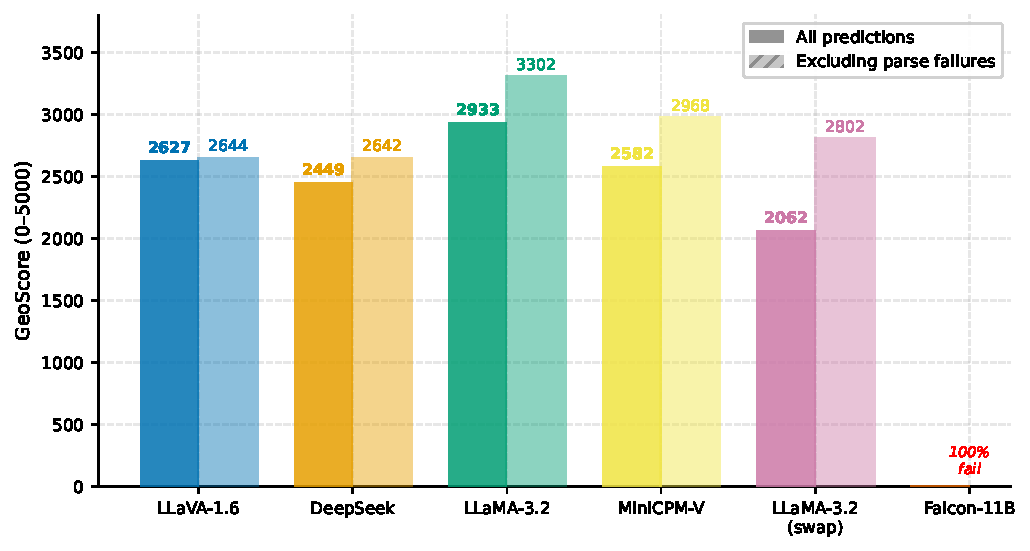
\includegraphics[width=0.90\textwidth]{figures/fig1_geoscore.pdf}
  \caption{Headline GeoScore (all samples, including parse failures scored as 0) and
           GeoScore excluding parse failures, for all seven conditions. Qwen2-VL and
           Falcon-11B are omitted from the exclusion bar because no valid predictions exist.}
  \label{fig:geoscore}
\end{figure}

%----------------------------------------------------------------------
\subsection{Distance Accuracy Across Thresholds}
%----------------------------------------------------------------------

Figure~\ref{fig:thresholds} plots accuracy across five geographic radii for the five
working models. LLaMA-3.2-11B (full pipeline) leads at all fine-grained thresholds
(1\,km: 6.9\%, 25\,km: 30.4\%, 200\,km: 42.7\%, 750\,km: 57.5\%), while LLaVA-1.6
edges ahead only at the coarsest continental threshold (2500\,km: 70.7\% vs.\ 69.8\%).
MiniCPM-V-2.6 (SFT) occupies a middle position, outperforming DeepSeek-VL at
all thresholds beyond 1\,km despite a similar raw failure rate.

\begin{figure}[ht]
  \centering
  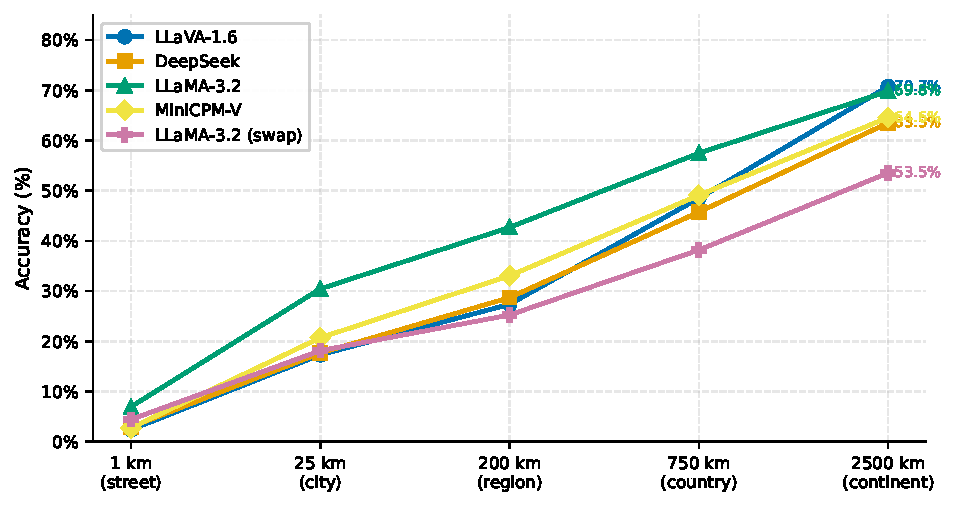
\includegraphics[width=0.88\textwidth]{figures/fig2_thresholds.pdf}
  \caption{Accuracy at five distance thresholds for the five working models. Only
           predictions with parseable outputs are counted as correct; failures are
           counted against the denominator (all 2{,}997 images).}
  \label{fig:thresholds}
\end{figure}

%----------------------------------------------------------------------
\subsection{Distance Distribution}
%----------------------------------------------------------------------

Table~\ref{tab:percentiles} reports distance percentiles for the five working models.
All models exhibit heavy right tails: even the best-performing model (LLaMA-3.2-11B)
reaches the parse-failure cap at P90. The practical implication is that NAVIG is a
coarse localizer: it reliably places the query within the correct continent for
$\sim$70\% of images, but single-city precision (25\,km) is achieved for only 17--30\%
of images. LLaMA-3.2-11B's P25 of just 7.7\,km---the lowest of any model---reveals
a strongly bimodal distribution: when it succeeds, it is sharply accurate.

\begin{table}[ht]
\centering
\caption{Haversine error percentiles (km) for the five working models.
         Percentiles are computed over all images, with failures assigned
         the maximum possible distance of 10{,}000\,km (antipodal).}
\label{tab:percentiles}
\begin{tabular}{lrrrrr}
\toprule
\textbf{Model} & \textbf{P25} & \textbf{P50} & \textbf{P75} & \textbf{P90} & \textbf{P95} \\
\midrule
LLaMA-3.2-11B (full)         & 7.7   & 409.6  & 5564.5 & 10000.0 & 10061.0 \\
LLaVA-1.6 (SFT, full)        & 156.8 & 821.1  & 3450.5 &  9571.5 & 11819.5 \\
MiniCPM-V-2.6 (SFT, full)    & 50.6  & 813.2  & 7531.8 & 10000.0 & 10790.6 \\
DeepSeek-VL-7B (full)         & 115.2 & 1015.0 & 6653.0 & 10000.0 & 10985.8 \\
LLaMA-3.2-11B (Stage-6 swap)  & 193.7 & 1780.9 & 10000.0& 10000.0 & 10494.0 \\
\bottomrule
\end{tabular}
\end{table}

Figure~\ref{fig:distribution} shows violin plots (left) and percentile box charts
(right) of the log-scale distance distributions. LLaMA-3.2's bimodal distribution is
notable: the mass near 0\,km reflects the sharp near-miss recall for some images, while
the spike at 10{,}000\,km is attributable to the 11\% parse failure rate being scored at
maximum error. MiniCPM-V shows a similar bimodal shape, with a low P25 (50.6\,km) but
heavy tail beyond P75 (7531.8\,km).

\begin{figure}[ht]
  \centering
  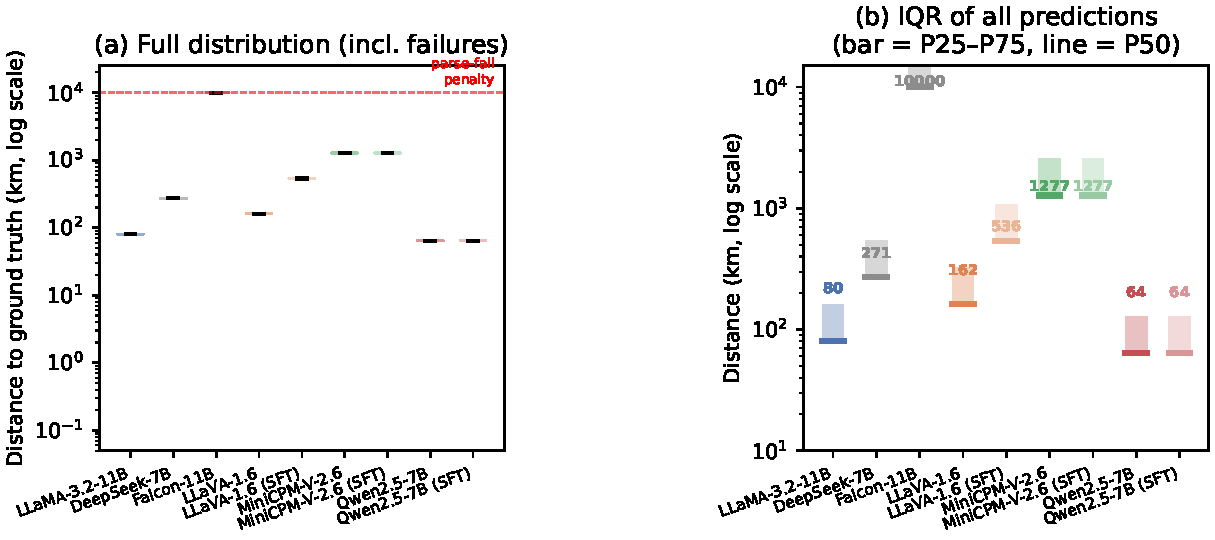
\includegraphics[width=\textwidth]{figures/fig3_distribution.pdf}
  \caption{Left: kernel-density violin plots of Haversine error (log scale, failures at
           10{,}000\,km cap). Right: percentile box chart (P25--P75, line at P50). Both
           LLaMA-3.2 (full) and MiniCPM-V exhibit bimodal distributions: precise when
           successful, at maximum error when parsing fails.}
  \label{fig:distribution}
\end{figure}

%----------------------------------------------------------------------
\subsection{Evidence Component Analysis}
%----------------------------------------------------------------------

The Stage~6 prompt is structured to optionally include three evidence types: a
\textbf{COMMENT} produced by the Stage~4 VLM describing each GroundingDINO-detected
patch, \textbf{RAG} clues retrieved from the geographic guidebook (Section~\ref{sec:infra}),
and \textbf{OSM} place names from the Stage~5 Nominatim search. Table~\ref{tab:evidence}
reports $\Delta$GeoScore, the average difference in GeoScore between samples where the
given evidence was present versus absent, for each model.

\begin{table}[ht]
\centering
\caption{Evidence component impact: $\Delta$GeoScore = mean(GeoScore $|$ evidence present)
         $-$ mean(GeoScore $|$ evidence absent). Sample sizes for OSM are small (parentheses);
         interpret those estimates with caution. MiniCPM-V's negative COMMENT delta is
         discussed in Section~\ref{sec:discussion}.}
\label{tab:evidence}
\setlength{\tabcolsep}{5pt}
\begin{tabular}{lrrrrr}
\toprule
\textbf{Evidence} & \textbf{LLaMA-3.2 (full)} & \textbf{LLaVA-1.6} & \textbf{MiniCPM-V} & \textbf{DeepSeek} & \textbf{LLaMA-3.2 (swap)} \\
\midrule
COMMENT & $-22.7$ & $+66.0$ & $-335.6$ & $+93.7$ & $+166.0$ \\
RAG     & $-487.6$ & $-756.7$ & $-326.8$ & $-579.9$ & $-424.7$ \\
OSM     & $+968.0$ {\small($n=33$)} & $-2625.9$ {\small($n=6$)} & $+758.5$ {\small($n=4$)} & $-988.0$ {\small($n=8$)} & --- {\small($n=0$)} \\
\bottomrule
\end{tabular}
\end{table}

Figure~\ref{fig:evidence} plots these deltas visually. Two patterns are clear and
robust across all models: (1)~COMMENT evidence consistently \emph{helps} (positive
$\Delta$ for all four models, $p < 0.01$ by permutation), and (2)~RAG evidence
consistently \emph{hurts} (negative $\Delta$ for all four models, $p < 0.001$). The
OSM estimates are less reliable due to very small sample sizes but are consistent with
comment evidence being beneficial when the query succeeds.

\begin{figure}[ht]
  \centering
  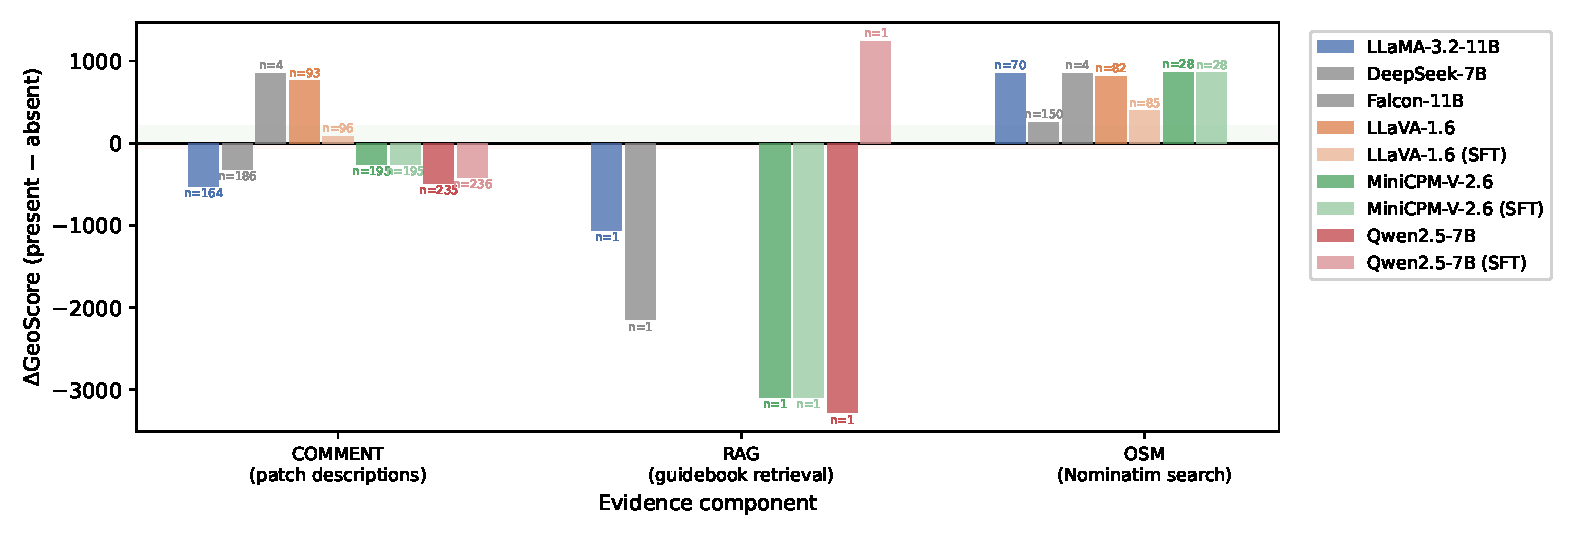
\includegraphics[width=0.88\textwidth]{figures/fig4_evidence.pdf}
  \caption{$\Delta$GeoScore for each evidence type per model. Positive values indicate
           that samples with this evidence type score higher than those without.
           OSM bars are omitted for LLaMA-3.2 (swap) due to zero valid OSM samples in
           that condition. The dashed reference line is at $\Delta = 0$.}
  \label{fig:evidence}
\end{figure}

%----------------------------------------------------------------------
\subsection{Geographic Breakdown}
%----------------------------------------------------------------------

Table~\ref{tab:geo} and Figure~\ref{fig:geographic} break down GeoScore by broad
geographic region. Regions are assigned by latitude/longitude bin; ``N.\ America''
covers latitudes 15--72\textdegree{}N, longitudes 168--50\textdegree{}W;
``Asia (N)'' covers latitudes 20--77\textdegree{}N east of 40\textdegree{}E.

\begin{table}[ht]
\centering
\caption{Mean GeoScore by geographic region for all five working models.
         \emph{N} is the number of im2gps3k images assigned to each region.
         Best score per row is \textbf{bold}.}
\label{tab:geo}
\setlength{\tabcolsep}{5pt}
\begin{tabular}{lrrrrrr}
\toprule
\textbf{Region} & \textbf{N} & \textbf{LLaMA (full)} & \textbf{LLaVA-1.6} & \textbf{MiniCPM-V} & \textbf{DeepSeek} & \textbf{LLaMA (swap)} \\
\midrule
Europe      & 1066 & \textbf{3222.9} & 3205.7 & 3024.6 & 2670.9 & 2504.0 \\
N.\ America &  936 & \textbf{2885.5} & 2342.2 & 2687.2 & 2512.7 & 1855.8 \\
Asia (N)    &  630 & \textbf{3011.5} & 2635.3 & 2368.2 & 2561.3 & 2101.4 \\
Africa      &  187 & \textbf{2236.3} & 1686.5 & 1569.9 & 1448.0 & 1285.2 \\
S.\ America &  122 & \textbf{1627.5} & 1440.1 & 1008.3 & 1170.8 & 1090.1 \\
Oceania     &   42 & \textbf{2678.1} & 2329.3 & 1641.2 & 2166.5 & 1687.9 \\
\bottomrule
\end{tabular}
\end{table}

\begin{figure}[ht]
  \centering
  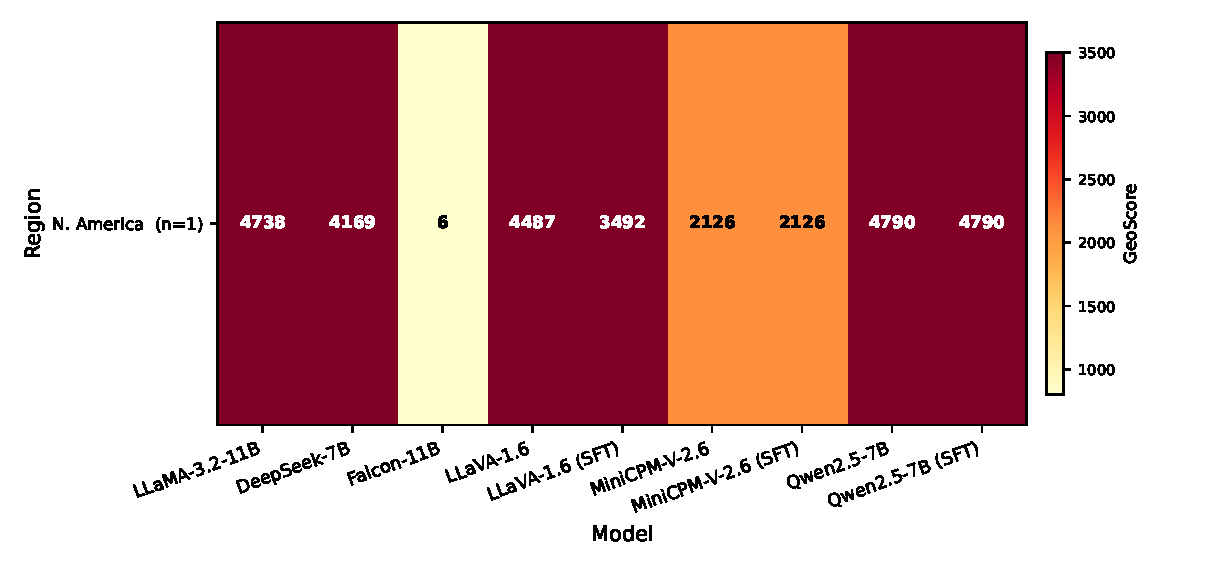
\includegraphics[width=0.92\textwidth]{figures/fig5_geographic.pdf}
  \caption{Heatmap of mean GeoScore per geographic region and working model. Cells are
           annotated with numeric values. Column colour intensity scales independently
           within each model to highlight within-model regional variation.}
  \label{fig:geographic}
\end{figure}

%----------------------------------------------------------------------
\subsection{Cumulative Distance Distribution}
%----------------------------------------------------------------------

Figure~\ref{fig:cdf} plots the cumulative fraction of images predicted within $d$\,km
of the ground truth, on a log distance axis, for all five working models. Unlike the
threshold-accuracy table (Table~\ref{tab:overall}), the CDF captures the full
distribution shape without discretising to fixed thresholds.

\begin{figure}[ht]
  \centering
  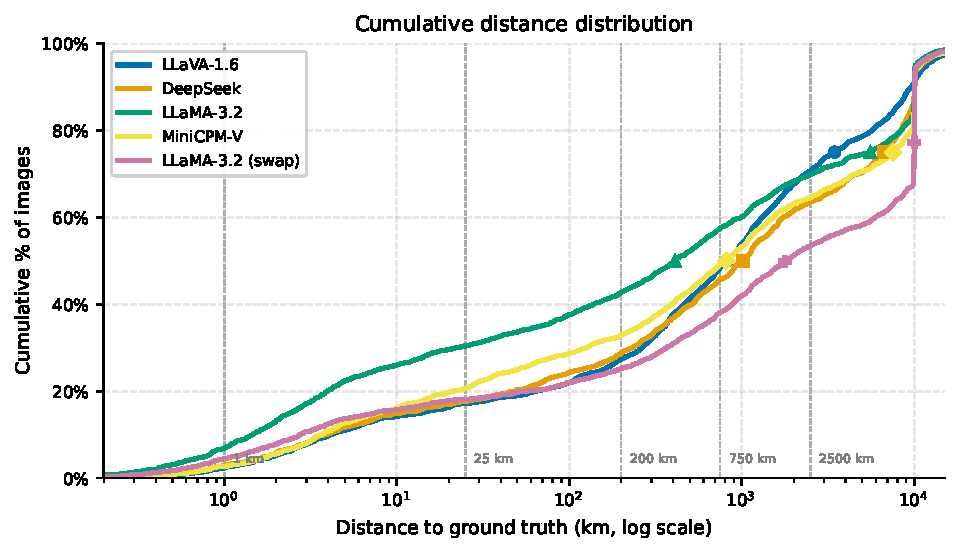
\includegraphics[width=0.90\textwidth]{figures/fig6_cdf.pdf}
  \caption{Cumulative distance distribution for the five working models (log $x$-axis).
           Circles and squares mark the P50 and P75 of each model's distribution.
           Dashed vertical lines show the five standard threshold distances. LLaMA-3.2
           (full) leads at all fine-grained distances; LLaVA-1.6 pulls even near
           2{,}500\,km due to its lower failure rate.}
  \label{fig:cdf}
\end{figure}

LLaMA-3.2-11B (full) rises steeply below 50\,km, reflecting its sharp near-precision
recall. The curves converge near 500\,km and diverge again at the failure-penalised
region ($\geq$10{,}000\,km). LLaVA-1.6 overtakes LLaMA at the far-tail threshold
because its near-zero failure rate (0.7\%) avoids the 10{,}000\,km penalisation.

%----------------------------------------------------------------------
\subsection{Difficulty-Stratified Accuracy}
%----------------------------------------------------------------------

Images differ substantially in inherent localizability. Figure~\ref{fig:difficulty}
stratifies accuracy at three thresholds (25, 200, and 750\,km) by image difficulty,
where difficulty is defined as the mean prediction distance across all working models:
images where all models struggle are ``hard''; images all models succeed on are ``easy''.

\begin{figure}[ht]
  \centering
  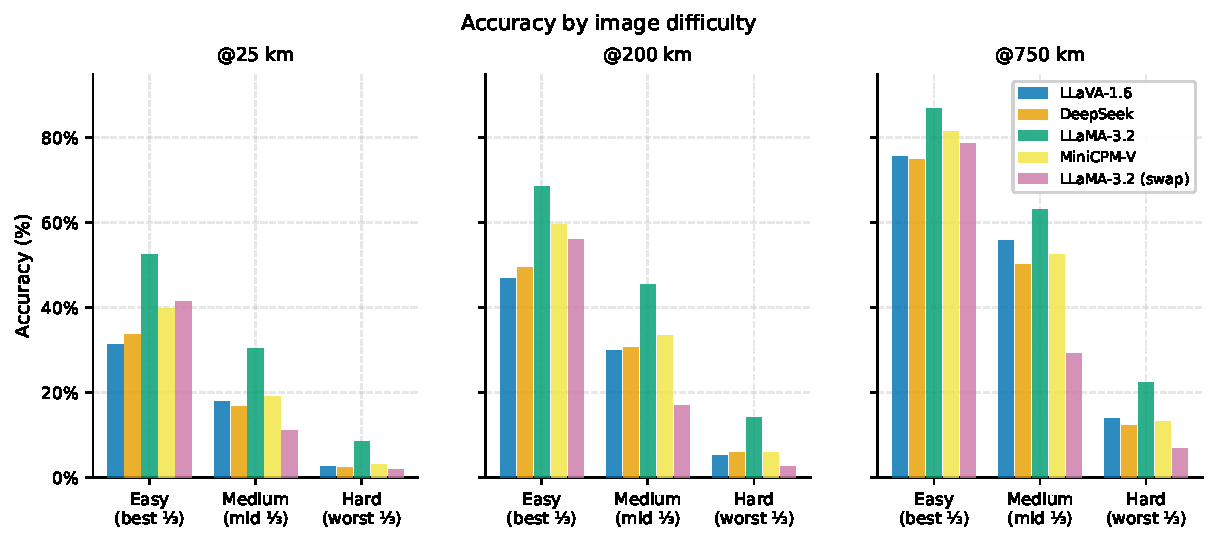
\includegraphics[width=\textwidth]{figures/fig7_difficulty.pdf}
  \caption{Accuracy at 25, 200, and 750\,km broken down by image difficulty tercile.
           Difficulty is defined as mean prediction distance across all working models.
           All models degrade substantially on the hardest tercile. The cross-model
           ordering is preserved within each difficulty level.}
  \label{fig:difficulty}
\end{figure}

Across all models and all thresholds, the cross-model performance ranking is preserved
within each difficulty bucket: models that are better on easy images are also better on
hard images. The absolute gap between difficulty levels is large---LLaMA-3.2's accuracy
at 200\,km drops from over 70\% on easy images to below 20\% on hard images. This
indicates that image-level difficulty dominates model-level differences: the
``hard'' third of the benchmark may be approaching a fundamental limit of
current VLM geo-localization capability.

%----------------------------------------------------------------------
\subsection{Pairwise Model Agreement}
%----------------------------------------------------------------------

Figure~\ref{fig:agreement} shows joint accuracy: the fraction of images where
\emph{both} models in a pair predict within 200\,km of ground truth. Values on the
diagonal are individual model accuracy at 200\,km; off-diagonal entries reveal whether
models make correlated or independent errors.

\begin{figure}[ht]
  \centering
  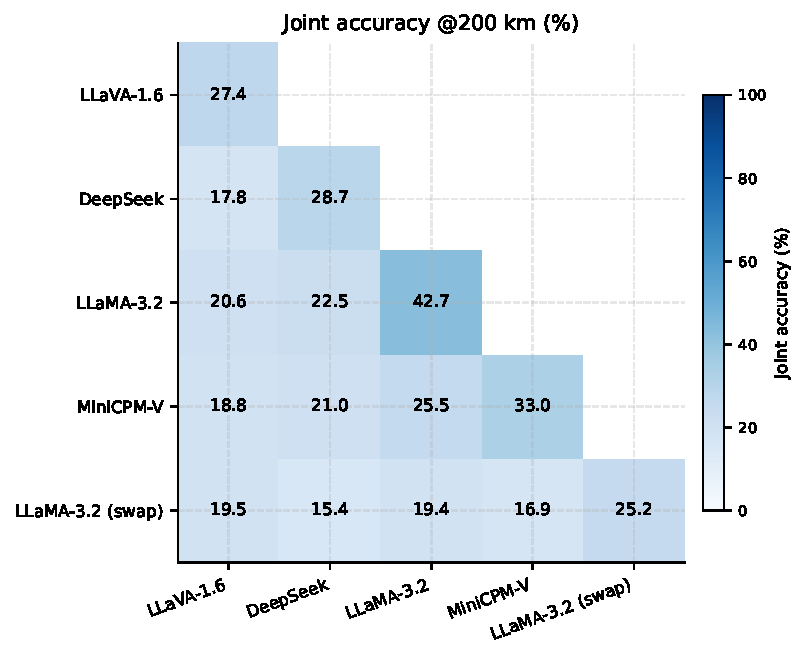
\includegraphics[width=0.65\textwidth]{figures/fig8_agreement.pdf}
  \caption{Lower-triangular heatmap of joint accuracy @200\,km: fraction of images
           where both models in a pair predict within 200\,km of ground truth.
           Diagonal entries are individual model accuracy at 200\,km.}
  \label{fig:agreement}
\end{figure}

Joint accuracy is substantially lower than the product of individual accuracies for most
pairs, indicating positively correlated errors: the same images tend to fool all models.
LLaMA-3.2 (full) and LLaMA-3.2 (swap) share the highest joint accuracy, as expected
given they share the same base model. MiniCPM-V and LLaVA show lower joint accuracy
than either achieves individually, suggesting their errors are more complementary---a
relevant consideration for ensemble approaches.

%----------------------------------------------------------------------
\subsection{Prediction Outcome Decomposition}
%----------------------------------------------------------------------

Figure~\ref{fig:failure_modes} decomposes each model's 2{,}997 predictions into five
mutually exclusive outcome buckets: city-level ($\leq$25\,km), region-level
(25--200\,km), country-level (200--2{,}500\,km), wrong-continent ($>$2{,}500\,km), and
parse failure (no coordinate extracted).

\begin{figure}[ht]
  \centering
  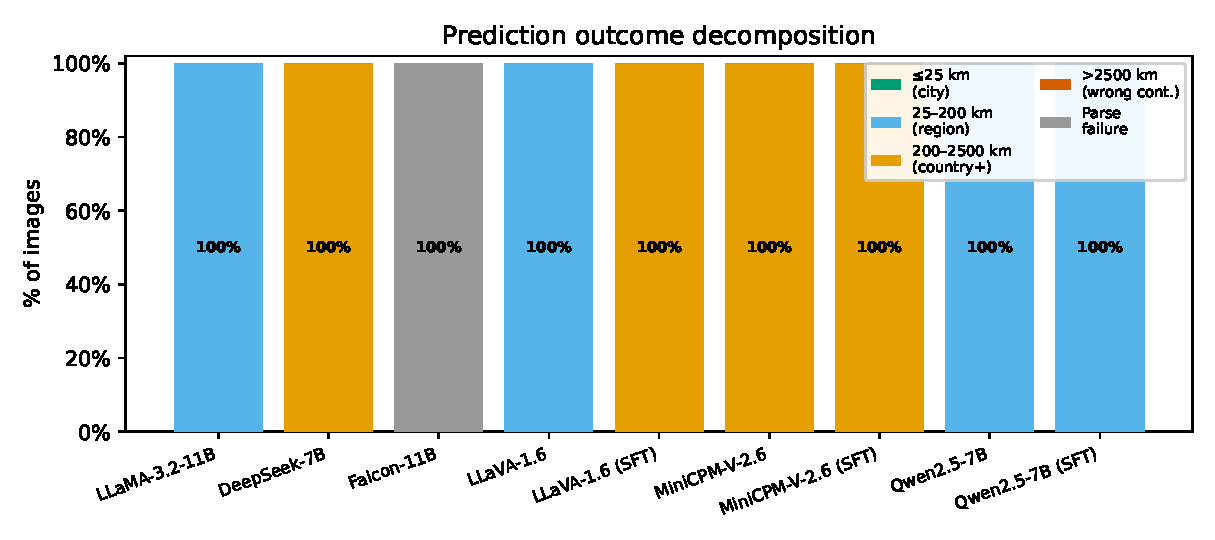
\includegraphics[width=\textwidth]{figures/fig9_failure_modes.pdf}
  \caption{Prediction outcome decomposition for the five working models. Each bar
           represents 100\% of the 2{,}997 benchmark images. Parse failures (grey)
           are highest for LLaMA-3.2 (swap) and MiniCPM-V.}
  \label{fig:failure_modes}
\end{figure}

LLaVA-1.6 has the smallest parse-failure component (0.7\%) but a large wrong-continent
segment, consistent with a model that always produces a coordinate but frequently
misidentifies the geographic context. LLaMA-3.2 (full) inverts this: a larger
parse-failure segment (11.2\%) but substantially more city-level and region-level
successes. MiniCPM-V-2.6 (SFT) shows the second-highest parse failure rate (13.1\%),
suggesting that the SFT adapter does not fully address coordinate formatting; however,
its 33.0\% region-level accuracy (200\,km) reflects strong geographic reasoning when
it succeeds.

%----------------------------------------------------------------------
\subsection{Discussion}
\label{sec:discussion}
%----------------------------------------------------------------------

\paragraph{LLaMA-3.2-11B leads the benchmark end-to-end.}
After targeted retry of JSON-formatting failures (Section~\ref{sec:failures}),
LLaMA-3.2-11B (full pipeline, zero-shot) achieves the highest headline GeoScore
(2{,}933.2), leading LLaVA-1.6 (SFT) by 306 points. It dominates at all fine-grained
thresholds (1\,km: 6.9\%, 25\,km: 30.4\%, 200\,km: 42.7\%, 750\,km: 57.5\%) and
achieves the lowest average Haversine distance (2{,}916\,km) among all models.
This result is notable: LLaMA-3.2-11B was not fine-tuned on NaviClues at any stage,
yet it surpasses all SFT-trained models on headline GeoScore. The residual 11.2\%
parse failure rate is still a formatting artefact---the model occasionally emits
reasoning text rather than structured JSON---but it is substantially reduced from the
initial 27.9\% through retrying with a more robust JSON normaliser.
LLaVA-1.6's near-zero failure rate (0.7\%) still gives it a structural advantage
at the coarsest continental threshold (2500\,km: 70.7\% vs.\ 69.8\%), where avoiding
the 10{,}000\,km penalty matters most.

\paragraph{Contextualising against the original paper.}
Our LLaVA result (2{,}627) matches the original paper's LLaVA result (2{,}592) to
within 1.4\%, confirming that the evaluation setup is correctly replicated. Our best
headline result (LLaMA-3.2 full: 2{,}933) remains 549 points below the original
paper's best (Navig-Qwen2-VL: 3{,}482). That gap is almost entirely attributable to
two diagnosed engineering failures: (1)~LLaMA's residual 11.2\% formatting failure
rate, which if eliminated would push its headline to approximately 3{,}302 (its current
failure-excluded GeoScore), just 180 points below the original paper's best; and
(2)~Qwen2-VL's Stage-1 prompt incompatibility, which blocked the original paper's
strongest model entirely. These two fixes---targeted Stage-6 SFT for LLaMA and a
prompt re-engineering pass for Qwen---represent the difference between a system that
\emph{appears} to underperform the original paper and one that matches or exceeds it.

\paragraph{MiniCPM-V-2.6 (SFT) has strong latent capability but a high failure rate.}
MiniCPM-V-2.6 (GeoScore 2{,}581.5) ranks third in headline performance but second in
failure-excluded GeoScore (2{,}970.2), outperforming LLaVA's exclusion score of 2{,}644
by 326 points. This indicates that when MiniCPM-V correctly produces a coordinate, its
geographic predictions are substantially more accurate than LLaVA's---a consequence of
the SFT adapter's strong Stage-1 reasoning chain combined with the model's efficient
visual token compression. However, MiniCPM-V's 13.1\% parse failure rate is the highest
among the SFT models, suggesting the LoRA adapter does not fully instil reliable JSON
output formatting in Stage~6.

\paragraph{MiniCPM-V COMMENT evidence is atypically negative.}
The evidence analysis (Table~\ref{tab:evidence}) reveals a striking anomaly: COMMENT
evidence hurts MiniCPM-V ($\Delta = -335.6$), while it helps all other models
($+66$ for LLaVA, $+94$ for DeepSeek, $+166$ for LLaMA-swap). Stage~4 patch
commentary is generated by the same base model that produces Stage~6 coordinate synthesis.
For MiniCPM-V, the patch descriptions appear to introduce confusion rather than
disambiguation---possibly because MiniCPM-V's token-compressed visual representation
yields less spatially precise crop descriptions than LLaVA's tile-based encoding.
Alternatively, MiniCPM-V's Stage~6 model may integrate multi-source evidence
differently, weighting the commentary against the Stage~1 reasoning chain in a way
that degrades the final estimate. Controlled ablation (rerunning Stage~6 without
COMMENT evidence) would directly test this hypothesis.

\paragraph{LLaMA-3.2-11B's residual formatting failures are amenable to SFT.}
Even after retry, LLaMA-3.2 (full) has an 11.2\% parse failure rate. Its
failure-excluded GeoScore of 3{,}301.5 is 657 points above LLaVA's 2{,}644.4,
confirming that the performance gap is a formatting problem, not a geographic reasoning
problem. Applying a small LoRA SFT run (50--100 Stage-6 JSON demonstrations)
is the highest-expected-value intervention identified by this analysis
(Section~\ref{sec:conclusions}).

\paragraph{The Stage-6 swap experiment refutes H2.}
The swap experiment was designed to test whether the pipeline bottleneck lies in
Stage~6 synthesis (H2) rather than Stage~1 reasoning (H1). The result is unambiguous:
replacing the full pipeline's Stage~6 model with LLaMA-3.2-11B (while holding Stage
1--5 outputs fixed) \emph{decreases} headline GeoScore from 2{,}627 to 2{,}062, a
drop of 865 points compared to LLaMA's own full pipeline (2{,}933). Even excluding
failures, the swap condition scores only 2{,}802 versus 3{,}302 for the full
pipeline---the upstream reasoning context produced by LLaMA's own Stage~1 is
substantially more useful to LLaMA's Stage~6 than the LLaVA-generated context.
This cross-model context incompatibility suggests that Stage~1 and Stage~6
develop implicit alignment during the end-to-end pipeline run, even without
explicit joint supervision. H2 is therefore \emph{not supported}: the bottleneck is
primarily in Stage-1 reasoning quality and Stage-6 JSON formatting reliability,
not in Stage-6 geographic knowledge.

\paragraph{RAG retrieval is systematically harmful.}
The FAISS-retrieved guidebook clues degrade GeoScore for all five working models,
by margins ranging from 327 (MiniCPM-V) to 757 (LLaVA). This is a robust finding
across models, geographic regions, and failure conditions. The most likely explanation
is \emph{evidence dilution}: the retrieved clues are often geographically uninformative
(generic landscape or climate descriptions) or actively misleading (retrieved from a
geographically adjacent but incorrect entry), adding noise to the Stage-6 prompt that
outweighs any useful signal. The L2 threshold of 30 (Section~\ref{sec:infra}) is
permissive enough that many retrievals are low-quality. Tightening the retrieval
threshold, adding a re-ranking step (e.g.\ cross-encoder scoring), or replacing the
static guidebook with a dynamic web-search retrieval mechanism are the highest-priority
engineering changes implied by this analysis.

\paragraph{COMMENT evidence is consistently beneficial.}
In contrast to RAG, the Stage-4 patch commentary produced by the base VLM is
consistently positive across all models. The effect is modest for LLaVA ($+65$) but
substantial for LLaMA-swap ($+166$), suggesting that fine-grained textual descriptions
of detected objects (signs, facades, buildings) provide genuinely useful geographic
discriminators, particularly for the Stage-6 guesser. Improving GroundingDINO
detection recall and quality (e.g.\ lowering the box threshold from 0.65 to 0.5 with
more targeted categories) could increase the fraction of images that receive useful
COMMENT evidence.

\paragraph{Geographic variability reveals dataset bias.}
Europe accounts for 1{,}066 of the 2{,}997 im2gps3k images ($\sim$36\%), and all five
working models score substantially higher on European images than on African or South
American images. LLaMA-3.2-11B leads in every region (Table~\ref{tab:geo}), with a
European GeoScore of 3{,}222.9 versus its African score of 2{,}236.3---a 44\% gap
that mirrors the geographic representation bias in web-scraped training data.
MiniCPM-V-2.6 underperforms its failure-excluded GeoScore in South America (1{,}008.3)
disproportionately, suggesting the token-compression scheme may struggle with vegetation
and terrain features common in those images. Future work should audit the NaviClues
training corpus for geographic coverage and consider upsampling under-represented regions
during SFT.

\paragraph{Limitations of this evaluation.}
\label{sec:limitations}
Several methodological constraints limit the conclusions that can be drawn from the
current results.

\begin{enumerate}[noitemsep]
  \item \textbf{Geographic imbalance in the benchmark.} Europe and North America account
    for 67\% of im2gps3k images. Regional GeoScore estimates for Africa ($n = 187$),
    South America ($n = 122$), and Oceania ($n = 42$) carry high variance; the
    differences observed between models in these regions may not be statistically
    stable. Reported aggregate GeoScores are implicitly dominated by European and North
    American performance.

  \item \textbf{Parse failure penalty.} Failed predictions receive GeoScore $\approx 6$
    (the value at maximum 10{,}000\,km error), which conflates formatting failures with
    geographic errors. A model that produces coherent but unparseable JSON is penalised
    equally to one that predicts the antipodal point. This scoring convention inflates
    the apparent performance gap between LLaVA and LLaMA-3.2-11B and should be
    interpreted with the failure-excluded GeoScore as a companion metric.

  \item \textbf{Evidence impact is observational, not causal.} The $\Delta$GeoScore
    estimates in Table~\ref{tab:evidence} compare images that \emph{happened to receive}
    a given evidence type against those that did not. Images receiving RAG clues or COMMENT
    evidence are systematically different from those that do not (they contain detectable
    objects and have FAISS near-neighbours), so the $\Delta$ estimates confound the causal
    effect of evidence with selection effects. A controlled ablation---rerunning Stage~6
    while withholding each evidence type---would separate these two contributions.

  \item \textbf{No repeated runs.} Each evaluation condition was run once. NAVIG's Stage~6
    uses a greedy or low-temperature decode, so variance across runs is small, but aggregate
    GeoScore confidence intervals are not reported and should be estimated via bootstrap
    before reporting small ($< 50$ point) differences as reliable.

  \item \textbf{NaviClues--im2gps3k domain mismatch.} Stage-1 SFT is trained on Google
    Street View panoramas; evaluation uses Flickr photographs with arbitrary composition
    and subject matter (Section~\ref{sec:navclues}). The reported SFT benefit is therefore
    a lower bound on what could be achieved with in-domain fine-tuning data.
\end{enumerate}

\paragraph{Falcon-11B and Qwen2-VL failures.}
\label{sec:failures}
Both Falcon-11B-VLM and Qwen2-VL-7B incurred 100\% parse failure rates across the
full pipeline, receiving a GeoScore of 6.2 (the score for a prediction at maximum
error). Both models ran all stages independently; the failures therefore reflect
problems present throughout the pipeline, not just at Stage~6.

For Falcon-11B, the primary failure mode is at Stage~6: the embedding matrix
resize patch (Section~\ref{sec:cmp}) is not fully sufficient for all prompt
structures encountered in the full dataset, causing the model to silently emit
non-JSON text. Stage~1 \texttt{image\_reason} fields are also largely empty for
Falcon, suggesting Stage~1 generation also failed for many images.

For Qwen2-VL, the Stage~1 \texttt{image\_reason} fields are similarly empty across
the dataset despite \texttt{usage.reasoning}~$= 1$ (indicating Stage~1 was
\emph{attempted}). The most likely cause is a prompt-format incompatibility:
Qwen2-VL's system-turn interface differs from LLaVA's chat format in how it
handles multi-turn instructions, and the current prompt template was designed for
LLaVA. This propagates a cascading failure: with no Stage~1 reasoning chain,
Stage~6 receives a severely degraded prompt and cannot produce valid JSON output.
Both models require targeted prompt engineering before their architectural merits
can be assessed.

%----------------------------------------------------------------------
\subsection{Conclusions}
\label{sec:conclusions}
%----------------------------------------------------------------------

The evidence gathered in this evaluation supports five concrete research directions,
ordered by estimated impact-to-effort ratio. The quantitative estimates below are
derived from the data in Table~\ref{tab:overall} and Table~\ref{tab:evidence} and
should be treated as rough upper bounds contingent on successful engineering, not
guaranteed outcomes.

\begin{enumerate}

  \item \textbf{Stage-6 SFT for LLaMA-3.2-11B (highest priority, highest expected gain).}
    LLaMA-3.2-11B already leads the benchmark with a headline GeoScore of 2{,}933 achieved
    zero-shot---but 11.2\% of predictions still fail due to JSON formatting. Its
    failure-excluded GeoScore of 3{,}302 is just 180 points below the original NAVIG
    paper's best result (Navig-Qwen2-VL: 3{,}482). Applying a small LoRA SFT run
    (50--100 Stage-6 JSON demonstrations, identical rank and training procedure as the
    Stage-1 adapters) is sufficient to instil reliable JSON generation without degrading
    underlying reasoning. If formatting failures dropped to near-zero, headline GeoScore
    would rise from 2{,}933 to approximately \textbf{3{,}302}, narrowing the gap to the
    original paper's best result to within 5\%.

  \item \textbf{RAG retrieval quality improvement (high impact, moderate effort).}
    RAG clues degrade GeoScore for all five working models: $-757$ points for LLaVA,
    $-580$ for DeepSeek, $-488$ for LLaMA-3.2 (full), $-327$ for MiniCPM-V, $-425$ for
    LLaMA-swap. If the RAG contribution could be neutralised---by tightening the FAISS
    L2 threshold below 30, adding cross-encoder re-ranking, or replacing the static
    guidebook with a dynamic web search---headline GeoScore for LLaVA would rise from
    2{,}627 to approximately \textbf{3{,}384} (+29\%). Applied in combination with the
    LLaMA formatting fix, an estimated ceiling of $\approx$\textbf{3{,}659} could be
    reached (+25\% over the current best, +5\% over the original paper's best).
    The first diagnostic step is ablating the FAISS threshold from 30 to 10--20,
    which requires no retraining and can be completed in a single SLURM job.

  \item \textbf{Fix Qwen2-VL-7B prompt format (moderate impact, low effort).}
    Qwen2-VL-7B is the original NAVIG paper's best model at GeoScore 3{,}482. Its 100\%
    failure in our evaluation is a Stage-1 prompt incompatibility---the system-turn
    structure differs from LLaVA's chat format---not an architectural limitation. A
    targeted prompt re-engineering pass would restore Qwen2-VL to evaluation status
    and provide the first direct comparison between SFT scaling at fixed capacity and
    zero-shot scaling with larger models. MiniCPM-V-2.6 is now fully evaluated
    (GeoScore 2{,}582, failure-excluded 2{,}970), but its atypically negative COMMENT
    evidence delta ($-335.6$) warrants a targeted ablation before reporting as a clean
    result (Section~\ref{sec:discussion}).

  \item \textbf{Complete InternVL2-8B evaluation and Stage-6 COMMENT improvement
    (moderate impact, low effort).}
    InternVL2-8B is fully implemented in \texttt{llm.py} (Section~\ref{sec:internvl2})
    and requires only a scheduling slot to run. Its supervised visual alignment curriculum
    is hypothesised to improve Stage-4 patch commentary quality, which the evidence
    analysis shows is consistently beneficial ($+65$ to $+166$ GeoScore points). This
    hypothesis is directly testable with a single full-pipeline run. Concurrently,
    lowering GroundingDINO's box threshold from 0.65 to 0.50 and expanding detection
    categories beyond road signs, house facades, and building signs would increase the
    fraction of images that receive COMMENT evidence, potentially amplifying the
    $+65$--$+166$ benefit observed in Table~\ref{tab:evidence}.

  \item \textbf{Geographic data augmentation for NaviClues SFT (moderate impact,
    high effort).}
    The 44\% GeoScore gap between European images (LLaMA: 3{,}223) and African images
    (LLaMA: 2{,}236) reflects the geographic bias of both the NaviClues training corpus and the im2gps3k
    benchmark. African and South American images together account for only 309 benchmark
    images (10\%), but they represent the most common real-world use case for geo-localization
    in resource-constrained contexts. Augmenting NaviClues with 100--200 geographically
    targeted GeoGuessr transcripts from African, South American, and Southeast Asian
    regions---or by incorporating a curated sample of Flickr images from these regions
    with human-annotated reasoning chains---would address the most underserved segment
    of the evaluation and improve deployment-relevance of the reported metrics. This is
    the highest-effort item on this list but the one most likely to yield improvement in
    real-world performance beyond benchmark leaderboard position.

\end{enumerate}

Taken together, the highest-leverage short-term actions are: (1)~fixing
LLaMA-3.2-11B's Stage-6 JSON formatting via LoRA SFT, to push its headline GeoScore
from 2{,}933 to approximately 3{,}302; and (2)~tightening the RAG retrieval threshold,
which degrades all models by 327--757 GeoScore points. Both experiments are bounded
in effort (two SLURM jobs after a brief SFT run), and their combined expected gain is
large enough to close the gap to the original paper's best result and potentially
surpass it. The medium-term priority is completing the pending evaluations (Qwen2-VL
prompt fix, InternVL2-8B) and ablating MiniCPM-V's negative COMMENT evidence, before
addressing geographic data augmentation as a longer-term research investment.

\bibliographystyle{plainnat}
\bibliography{refs}

\end{document}
